
\chapter{The (One) Way to Proceed for Getting a Reasonable Design}

\section{General Considerations}

There are multiple strategies to develop a software application, though basically all of them comprise the following four phases:
\begin{enumerate}
    \item establish the \textit{application requirements} or specification;
    \item derive the ways the requirements can be realized / satisfied, i.e. \textit{designing} the application;
    \item \textit{implement} the design, e.g. write the corresponding code;
    \item check if the implementation satisfies the specification, at least by \textit{testing} (as exhaustive as possible) the developed application.
\end{enumerate}

In practice, a perfect and complete design is not entirely possible from the beginning for most of the projects. So, at least the last three phases actually correspond to a progressive and repeating process, i.e. make a first design, implement it, test the resulting code, see what is working bad or missing functionality, go back and change the design, make the corresponding code changes or additions, test them again and so on. 

I want, however, to warn you that even if we cannot make a perfect design from the beginning that does not mean that we do not have to make any design at all and just start writing code. This is a really bad idea. And actually, in my opinion, when you start writing code without a more or less formal design, what you actually have to do is to derive an on-the-fly design. What I mean is that you cannot just write ``some'' code there, hoping to get the required functionality. You must think of \textit{how} to code and \textit{what} code to write and this is basically a (hopefully, logical) plan, i.e. a design. Such a strategy, however, results most of the time and for most of the people in just poorly improvisation and requires many returns to the ``design'' phase to change data structures and code. In short, a lot of lost time and bad results. 

Coming back to the idea that we cannot make a complete design from the beginning, there are a few ways to understand this and reasons of having it. Firstly, it is generally difficult to cover all the particular cases, especially for very complex systems and requirements. That means that what you get first is a sort of a general design, establishing the main components of your application and their basic interrelationships. It is not surely that you immediately could start writing code for such a design, but it is very possible to be able to write some prototype, just to see if your ideas and design components could be linked together. On way or another, the next major step is to go deeper for a more detailed design. Secondly, one reason of not getting a complete design from the beginning is just because you want to concentrate on a particular component firstly, and only than to cope with the others. However, this is just a particular case of the first strategy, because it is not possible to deal with one application component without knowing firstly which are the others and how they depend on one another. Thirdly, maybe it is not needed to get a complete detailed design from the beginning, just because the application components are dealt with by different teams or, like in your case, different team members. It is not needed in such a case to deal with the complexity of each application component from the beginning, as each one be will be addressed latter by its allocated team (members), but just try to establish as precise as possible, which are the application components and how they need to interact each other. In your \OSName{} project the application components are most of the time already established, so what remains for you is only to clarify the interactions and interfaces between them. After such a general design, each team (member) can get independently into a more detailed design of his/her allocated application component. 
In conclusion, you need to derive at least a general design before starting writing any code and refine that design later. 

Take into  account, however, that in or project we have distinct deadlines for both design and implementation phases, and that you will be graded for the two relatively independent (thus, design regrading will be done only occasionally). This means that you have to try to derive a very good and as detailed as possible design from the beginning.  


Another practical idea regarding the application development phases is that there is no clear separation between those phases and especially between the design and implementation ones. This means that during what we call the design phase we have to decide on some implementation aspects and, similarly, when we are writing code we still have to take some decisions when more implementation alternatives exists (which could influence some of the application non-functional characteristics, like performance) or some unanticipated problems arise. Even taking into account such realities, in this design document we are mainly interested (and so you have to focus) mainly on the design aspects. But, as I said above, I will not expect you providing a perfect design, which would need no changes during its implementation. However, this does not mean that you are free to come with an unrealistic, incoherent, illogical, hasty, superficial design, which does not deal with all the (clear and obvious) given requirements. 

One important thing to keep in mind when you make your design and write your design document is that another team member has to be able to figure out easily what you meant in your design document and implement your design without being forced to take any additional design decisions during its implementation or asking you for clarifications. It is at least your teacher you have to think of when writing your design document, because s/he has to understand what you meant when s/he will be reading your document. Take care that you will be graded for your design document with approximately the same weight as for your implementation. 

Beside the fact that we do not require you a perfect design, and correspondingly we do not grade with the maximum value only perfect designs (yet, please, take care and see again above what I mean by an imperfect design), your design document must also not be a formal document. At the minimum it should be clear and logical and complies the given structure, but otherwise you are free to write it any way you feel comfortable. For example, if you think it helps someone better understand what you mean or helps you better explain your ideas, you are free to make informal hand-made figures, schemes, diagrams, make a photo of them or scan them and insert them in your document. Also, when you want to describe an algorithm or a functionality, you are free to describe it any way it is simpler for you, like for instance as a pseudo-code, or as a numbered list of steps. However, what I generally consider a bad idea is to describe an algorithm as an unstructured text. On one hand, this is difficult to follow and, on the other hand, text could generally be given different interpretations, though as I already mentioned your design should be clear and give no way for wrong interpretation, otherwise it is a bad design. 

Regarding the fact that design and implementation could not be clearly and completely separated, this is even more complicated in your \OSName{} project that you start from a given code of an already functional system. In other words you start with an already partially designed system, which you cannot ignore. This means, on one hand, that you could be restricted in many ways by the existing design and \OSName{} structure and, on the other hand, that you cannot make your design ignoring the \OSName{}' code. Even if, theoretically, a design could be abstract enough to support different implementations (consequently, containing no particular code), your \OSName{} design has to make direct references to some existing data structures and functions, when they are needed for the functionality of the \OSName{} component your are designing. So, do not let your design be too vague (abstract) in regarding to the functionality directly relying on exiting data structures and functions and let it mention them explicitly. For instance, when you need to keep some information about a thread, you can mention that such information will be stored as additional fields of the ``\textit{THREAD}'' data structure. Or, when you need to keep a list of some elements, you have to use the lists already provided by \OSName{} and show that by declaring and defining your list in the way \OSName{} does, like below:

\begin{lstlisting}
	// this is the way HAL9000 declares a generic list
	LIST_ENTRY myCoolList;

	typedef struct _MY_LIST_ELEM {
		... some fields ...

		// this is needed for linking MY_LIST_ELEM in the 
		// myCoolList list
		LIST_ENTRY ListElem;
	} MY_LIST_ELEM, *PMY_LIST_ELEM;
\end{lstlisting}

The next sections illustrate the design document structure we require and describe what each section should refer to.


\section{Application Requirements. Project Specification}

% Describe briefly what you have been given (have started from) at the beginning of the assignment and the way the existing functionality must be extended.

\subsection{``What you have'' and  ``What you have to do''}

In this section you have to make clear what you are required to do for each particular assignment of the \OSName{} project. In the \OSName{} project, you are already given the assignment requirements, so it is not your job to establish them. You must, however, be sure that you clearly understand them. Having no clear idea about what you have to do, gives you a little chance to really get it working. Please, do not hesitate to ask as many questions about such aspects on the \OSName{} forum (on the moodle page of the course) as you need to make all the requirements clear to you. Take care, however, that you have to do this (long enough) before the design deadline, such that to get an answer in time. We will do our best in answering your questions as fast as possible, though we cannot assure you for a certain (maximum) reaction time. You will not excused at all if you say you had not understood some requirements when you will be presenting your design document.

So, for this small section, take a moment and think of and briefly write about: 
\begin{enumerate}
    \item what you are starting from, i.e. what you are given in terms of \OSName{} existing functionality, and
    \item what you are required to do.
\end{enumerate}


\subsection{``How it would be used''}

Making clear the requirements could be helped by figuring some ways the required functionality would be used once implemented. 
For this you have to describe briefly a few common use-cases, which could later be used as some of the implementation tests. 

You could use for this the tests provided with the \OSName{} code in the ``tests/'' subdirectory. Take at least a short look at each test case to identify common cases.


\section{Derive the Application's Design}

Generally, you have to follow a top-down design approach, starting with a particular requirement and identifying the inputs it generates to your application (i.e. \OSName{} OS). Such that you could establish the ``entry (starting) points'' in your system to start your design from. 

Next, you also have to identify the logical objects (i.e. data structures, local and global variables etc.) implied and affected by the analyzed requirement and the operations needed to be performed on them. Also establish if you need to introduce and use additional information (i.e. fields, variables) in order to make such operations possible. 

Once you established the information you need to keep in order to dealt with the analyzed requirement, you could decide on the way to keep track of and manage that data. 
In other words, this is the way you can \textit{identify the needed data structures} and \textit{operations on them}. There could not necessarily be just one solution. For example, at one moment you could use a linked list or a hash table. In order to decide for one or another, you have to figure out which one helps you more, which one fits better for the most frequent operation and other things like these. Once you decided on the data structures, you have to establish where and how they are
\begin{inparaenum}[(1)]
    \item \textit{initialized}, 
    \item \textit{used}, 
    \item \textit{changed}, and finally 
    \item \textit{removed}.
\end{inparaenum}

This way you could identify the places (e.g. other system components, functions) where you have to add the needed functionality. In terms of \OSName{} code you could identify the functions needed to be used, changed or even added. 

As a result of your requirement analysis you could organize your resulting design like below. 

\subsection{Needed Data Structures and Functions}

Describe the \textit{data structures} and \textit{functions} (only their signature and overall functionality) needed by your design and what they are used for. Describe in few words the purpose of new added data structures, fields and functions. As mentioned before, cannot ignore the fact that \OSName{} is written in C. Thus, describe you data structures in the C syntax referring, when the case, to existing data structures, like in the example given above. If you only need to add new fields in existing data structures, mention only the added fields, not all of them. 

\begin{lstlisting}
    typedef struct _EXISTENT_DATA_STRUCTURE {
        ...
        int NewField;
        char NewField2;
        ...
    } EXISTENT_DATA_STRUCTURE, *PEXISTENT_DATA_STRUCTURE;
    
    typedef struct _NEW_DATA_STRUCTURE {
        ... new fields ...
    } NEW_DATA_STRUCTURE, *PNEW_DATA_STRUCTURE;
    
    STATUS NewFunction(void);
\end{lstlisting}


\subsection{Detailed Functionality}

This should be \textbf{the largest and most important section} of you design document. It must describe \textbf{explicitly}, in words and pseudo-code the way your solution works. DO NOT INCLUDE CODE HERE. This is a design document, not a code description one. As much as possible try to describe the design principles, not implementation details. 

Give examples, if you think they can make your explanation clearer. You are free to use any other techniques (e.g. use-case diagrams, sequence diagrams etc.) that you think can make your explanation clearer. See Figure~\ref{fig:sample-image} below to see the way images are inserted in a Latex file. 

\begin{figure}[h]
	\centering
	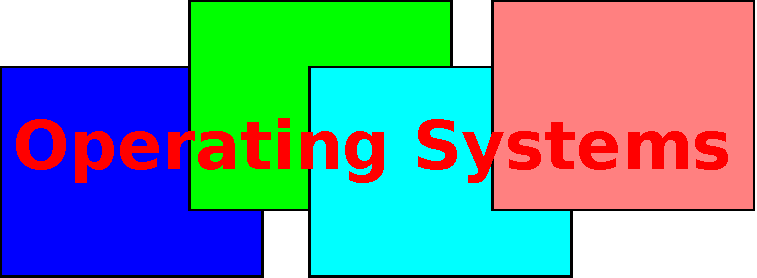
\includegraphics[width=0.5\textwidth]{figures/sample-image.pdf}
	\caption{Sample image}
	\label{fig:sample-image}
\end{figure}

When describing algorithms you are to use or develop, it is very important to also describe them in a formal way, not just as free text description. Commonly, this could be done as a sort of pseudo-code or just as a simple list of logically ordered steps (enumerated list). In your algorithm description you should (i.e. must) refer to the data structures and variables you described in the previous section, following the recommendations in Section~\ref{sec:derive-design}. This way you avoid describing your algorithms too vague and reduce the risks of being misunderstood.  

Here you have a pseudo-code description of an algorithm taken from \\ \href{http://en.wikibooks.org/wiki/LaTeX/Algorithms\_and\_Pseudocode\#Typesetting\_using\_the\_program\_package}{http://en.wikibooks.org/wiki/LaTeX}. It uses the \textit{algpseudocode} package. Alternatively, you can use any other package and environment of same sort you like. 

% \begin{program}
% \mbox{Example of a pseudo-code algorithm description:}
% \BEGIN
%   \FOR i:=1 \TO 10 \STEP 1 \DO
%      |expt|(2,i); \\ |newline|() \OD
% \rcomment{This text will be set flush to the right margin}
% \WHERE
% \PROC |expt|(x,n) \BODY
%           z:=1;
%           \DO \IF n=0 \THEN \EXIT \FI;
%              \DO \IF |odd|(n) \THEN \EXIT \FI;
% \COMMENT{This is a comment statement};
%                 n:=n/2; x:=x*x \OD;
%              \{ n>0 \};
%              n:=n-1; z:=z*x \OD;
%           |print|(z) \ENDPROC
% \END
% \end{program}

\begin{algorithmic}
\If {$i\geq maxval$}
    \State $i\gets 0$
\Else
    \If {$i+k\leq maxval$}
        \State $i\gets i+k$
    \EndIf
\EndIf
\end{algorithmic}

\subsection{Explanation of Your Design Decisions}

Justify very briefly your design decisions, specifying other possible design alternatives, their advantages and disadvantages and mention the reasons of your choice. For instance, you can say that you decided for a simpler and easier to implement alternative, just because you had no enough time to invest in a more complex one. Or just because you felt it would be enough for what \OSName{} tests would check for. This could be viewed as a pragmatical approach and it is not necessarily a bad one, on the contrary, could be very effective in practice.  


\section{Testing Your Implementation}

Please note that the \OSName{} code is provided with a set of tests that are used to check and evaluate your implementation. The \OSName{} tests could be found in the ``tests/'' subdirectory, organized in different subdirectories for each different assignments (like, ``threads'', ``userprog'' etc.).

To find out the names of all the tests to be run for a module you can build the \textit{RunTests} project and wait for execution to finish.

Actually, this is the first command that will be executed on your implementation when graded, so please, do not hesitate do run it by yourself as many times as needed during your \OSName{} development, starting from the design phase. 

In this section you have to describe briefly each of the given \OSName{} tests that will be run in order to check the completeness and correctness of your implementation. 
Take care that your grade is directly dependent on how many tests your implementation will pass, so take time to see if your design take into account all particular usage scenarios generated by all \OSName{} tests. 


\section{Observations}

You can use this section to mention other things not mentioned in the other sections. 

You can (realistically and objectively) indicate and evaluate, for instance:
\begin{itemize}
	\item the most difficult parts of your assignment and the reasons you think they were so; 
	
	\item the difficulty level of the assignment and if the allocated time was enough or not; 

	\item particular actions or hints you think we should do for or give to students to help them better dealing with the assignments.

\end{itemize}

You can also take a minute to think what your achieved experience is after finishing your design and try to share that experience with the others. 

You can also make suggestions for your teacher, relative to the way s/he can assist more effectively her/his students.

If you have nothing to say here, please remove it.
